\chapter{Introduction}
In this part of the dissertation we will discuss the improvements over
previous work \cite{previouswork}, both in terms of alternative tools
with respect to the ones presented in that thesis, and in terms of additional
areas where we can search for vulnerabilities.\\\\
In particular we will discuss how to gain access to the target network and list the
various programs that already exist for this purpose. We will also talk about
an extension to the previous work that allows to retrieve the memory image
of the target device and analyze it offline, aiming to find useful information
about what processes were running on said device and inspecting their memory.\\\\
Finally we will discuss what scripts were developed to automate the process
and how to use them in practice, but leaving the actual testing to the second part
of the thesis, and focusing only on their options and requirements.\\\\
\subsection{Attack description}
We will assume the attacker needs to perform the following steps:
\begin{enumerate}
    \item Gain access to the target network
    \item Search for the target device between the devices connected to the network
    \item Scan the device for open ports and understand what services are running
    \item Sniff the network traffic, both of the device and of the related app
    \item Analyze the traffic, to understand what protocols are used and try to
          extract information to continue the attack
    \item Try to retrieve the firmware of the device
    \item If the firmware is successfully downloaded, analyze it to find vulnerabilities
    \item Emulate the firmware or gain access to the real device to extract and
            analyze its memory
\end{enumerate}
During the test, the steps from 1 to 3 will be performed also in the
case of an uncofigured device, to understand if it is vulnerable
when not already fully functional, while the last ones will be performed only
if the device is configured.\\\\
In our model the attacker will have access to the device's network, so it is
possible to work locally, not having to worry about remote attacks.\\
The attacker will be equipped with a laptop running Kali Linux, or any other
similar distribution, so all the tools we will use are already installed by default,
or can be easily installed with the package manager.\\
The procedure is described graphically in \textbf{Figure \ref{fig:attack_procedure}}.
\newpage
\begin{figure}[h]
    \centering
    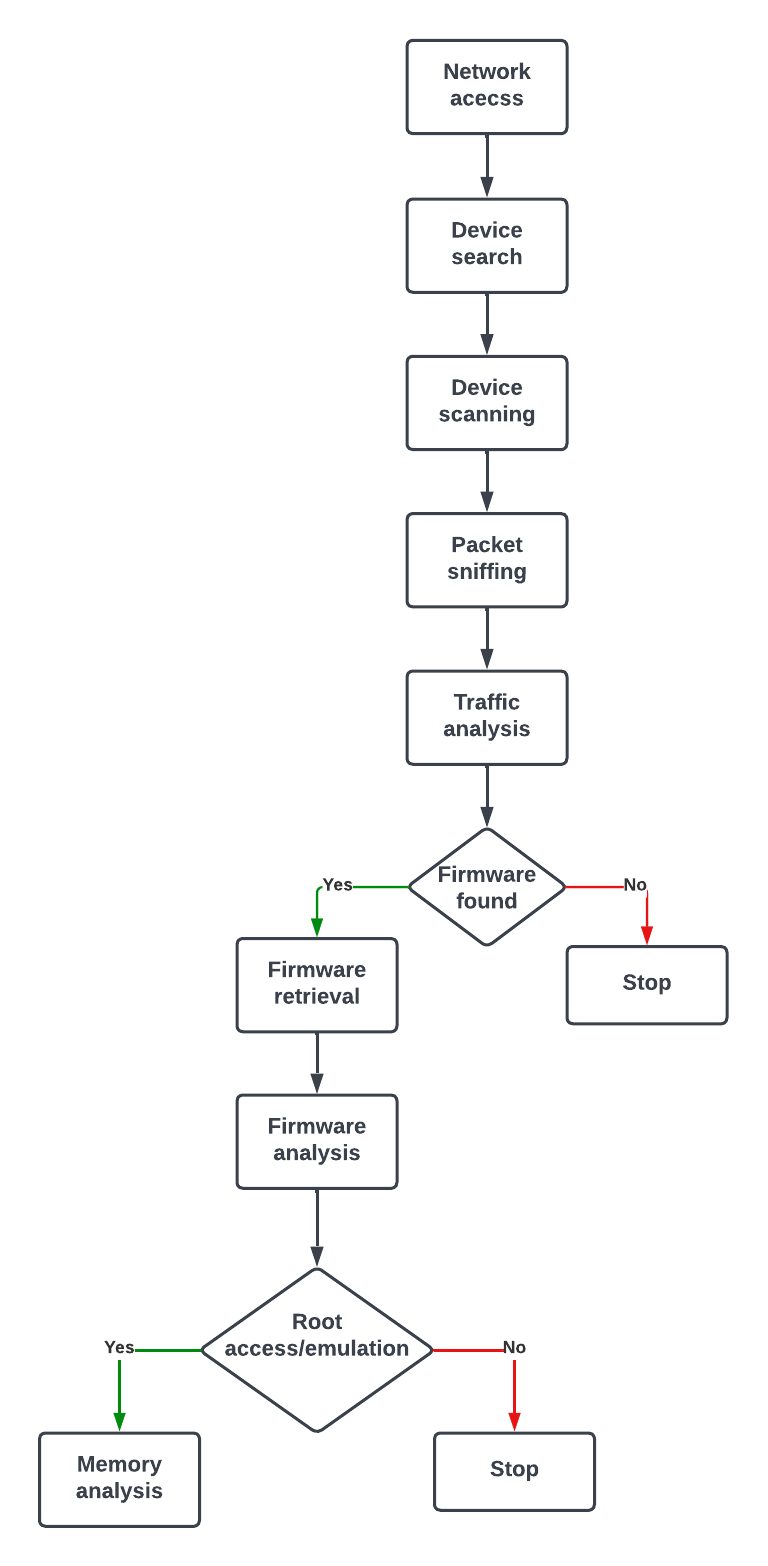
\includegraphics[scale=0.34]{Attack_procedure.png}
    \caption{Attack procedure}
    \label{fig:attack_procedure}
\end{figure}
\newpage